\documentclass[10pt]{beamer}
\usepackage[utf8]{inputenc}
\usepackage{xeCJK}
\usepackage{graphicx}
\usepackage {mathtools}
\usepackage{utopia}
\usepackage{booktabs}
\usepackage{tabularx}
\usepackage{tikz}
\usetikzlibrary{arrows.meta,positioning,fit,shapes.geometric}
\usetheme{CambridgeUS}
\usecolortheme{dolphin}

% set colors
\definecolor{myNewColorA}{RGB}{118,193,188}
\definecolor{myNewColorB}{RGB}{106,172,150}
\definecolor{myNewColorC}{RGB}{94,150,218}
\definecolor{softPanel}{RGB}{246,250,252}
\definecolor{softLine}{RGB}{185,202,218}
\definecolor{darkInk}{RGB}{31,41,55}
\definecolor{mutedInk}{RGB}{82,91,105}
\definecolor{warningRed}{RGB}{206,75,75}
\setbeamercolor*{palette primary}{bg=myNewColorC}
\setbeamercolor*{palette secondary}{bg=myNewColorB, fg=white}
\setbeamercolor*{palette tertiary}{bg=myNewColorA, fg=white}
\setbeamercolor*{titlelike}{fg=myNewColorA}
\setbeamercolor*{title}{bg=myNewColorA, fg=white}
\setbeamercolor*{item}{fg=myNewColorA}
\setbeamercolor*{caption name}{fg=myNewColorA}
\usefonttheme{professionalfonts}
\usepackage{natbib}
\usepackage{hyperref}

\setbeamertemplate{navigation symbols}{}
\titlegraphic{\includegraphics[height=1.5cm]{figures/hkulogo.png}}

\setbeamerfont{title}{size=\large}
\setbeamerfont{subtitle}{size=\small}
\setbeamerfont{author}{size=\small}
\setbeamerfont{date}{size=\small}
\setbeamerfont{institute}{size=\small}
\setbeamerfont{frametitle}{size=\large}
\title[FinSight]{FinSight}
\subtitle{ARIN7012 Project: Evidence-First Financial Analysis Chatbot}
\author[Group 4.2]{Group 4.2}

\institute[HKU]{The University of Hong Kong}
\date[ARIN7012 Presentation]{ARIN7012 Project Presentation}

\AtBeginSection[]{}

\tikzset{
  box/.style={draw=softLine, rounded corners=2pt, fill=softPanel, align=center, minimum height=0.72cm, text width=2.35cm, font=\scriptsize},
  mainbox/.style={box, draw=myNewColorC, fill=myNewColorC!10},
  greenbox/.style={box, draw=myNewColorB, fill=myNewColorB!12},
  tealbox/.style={box, draw=myNewColorA, fill=myNewColorA!14},
  redbox/.style={box, draw=warningRed, fill=warningRed!8},
  smallbox/.style={draw=softLine, rounded corners=2pt, fill=softPanel, align=center, minimum height=0.52cm, text width=1.75cm, font=\tiny},
  flow/.style={-{Latex[length=2mm]}, thick, draw=mutedInk},
  softflow/.style={-{Latex[length=2mm]}, draw=mutedInk}
}

\newcommand{\metric}[3]{%
  \begin{minipage}{0.18\textwidth}
    \centering
    {\Large\bfseries\textcolor{myNewColorC}{#1}}\\[-0.15em]
    {\scriptsize #2}\\[-0.1em]
    {\tiny\textcolor{mutedInk}{#3}}
  \end{minipage}
}
\newcommand{\slidenote}[1]{{\scriptsize\textcolor{mutedInk}{#1}}}

\begin{document}

\frame{\titlepage}

\section{Background and Goal}

\begin{frame}{Financial chatbot answers must be grounded}
  \begin{columns}[T,onlytextwidth]
    \column{0.48\textwidth}
      \begin{itemize}
        \item Finance questions may affect buy, hold, or sell decisions.
        \item User intent is often hidden inside short natural language.
        \item Market data, news, and macro signals change quickly.
        \item Answers need traceable evidence and clear limitations.
      \end{itemize}
    \column{0.48\textwidth}
      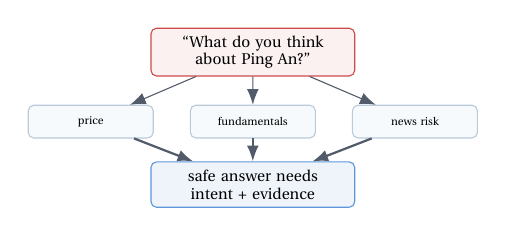
\begin{tikzpicture}[node distance=0.45cm, scale=0.80, transform shape]
        \node[redbox, text width=3.0cm] (q) {``What do you think about Ping An?''};
        \node[smallbox, below left=0.45cm and -0.05cm of q] (a) {price};
        \node[smallbox, below=0.45cm of q] (b) {fundamentals};
        \node[smallbox, below right=0.45cm and -0.05cm of q] (c) {news risk};
        \node[mainbox, below=1.35cm of q, text width=3.0cm] (out) {safe answer needs\\intent + evidence};
        \draw[softflow] (q) -- (a);
        \draw[softflow] (q) -- (b);
        \draw[softflow] (q) -- (c);
        \draw[flow] (a) -- (out);
        \draw[flow] (b) -- (out);
        \draw[flow] (c) -- (out);
      \end{tikzpicture}
  \end{columns}
\end{frame}

\begin{frame}{The project goal is an evidence-first financial chatbot}
  \begin{columns}[T,onlytextwidth]
    \column{0.48\textwidth}
      \begin{itemize}
        \item Understand product type, entities, intent, topic, and risk.
        \item Search likely answer sources: price, news, fundamentals, macro.
        \item Analyze numerical and text evidence before response generation.
        \item Produce answer JSON and next-question suggestions for the chatbot.
      \end{itemize}
    \column{0.48\textwidth}
      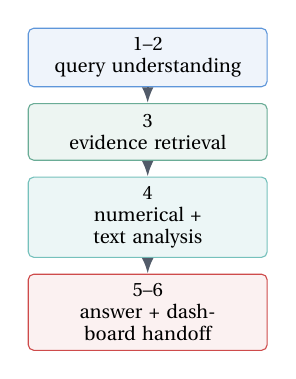
\begin{tikzpicture}[node distance=0.28cm]
        \node[mainbox, text width=2.8cm] (o1) {1--2\\query understanding};
        \node[greenbox, below=0.2cm of o1, text width=2.8cm] (o2) {3\\evidence retrieval};
        \node[tealbox, below=0.2cm of o2, text width=2.8cm] (o3) {4\\numerical + text analysis};
        \node[redbox, below=0.2cm of o3, text width=2.8cm] (o4) {5--6\\answer + dashboard handoff};
        \draw[flow] (o1) -- (o2);
        \draw[flow] (o2) -- (o3);
        \draw[flow] (o3) -- (o4);
      \end{tikzpicture}
  \end{columns}
\end{frame}

\begin{frame}{FinSight is powered by the ARIN intelligence backend}
  \centering
  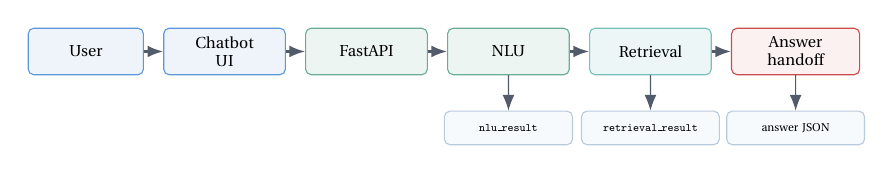
\begin{tikzpicture}[node distance=0.32cm, scale=0.82, transform shape]
    \node[mainbox, text width=1.55cm] (u) {User};
    \node[mainbox, right=0.3cm of u, text width=1.65cm] (chat) {Chatbot\\UI};
    \node[greenbox, right=0.3cm of chat, text width=1.65cm] (api) {FastAPI};
    \node[greenbox, right=0.3cm of api, text width=1.65cm] (nlu) {NLU};
    \node[tealbox, right=0.3cm of nlu, text width=1.65cm] (ret) {Retrieval};
    \node[redbox, right=0.3cm of ret, text width=1.75cm] (ans) {Answer\\handoff};
    \node[smallbox, below=0.55cm of nlu, text width=1.75cm] (nj) {\texttt{nlu\_result}};
    \node[smallbox, below=0.55cm of ret, text width=1.9cm] (rj) {\texttt{retrieval\_result}};
    \node[smallbox, below=0.55cm of ans, text width=1.9cm] (aj) {answer JSON};
    \draw[flow] (u) -- (chat);
    \draw[flow] (chat) -- (api);
    \draw[flow] (api) -- (nlu);
    \draw[flow] (nlu) -- (ret);
    \draw[flow] (ret) -- (ans);
    \draw[softflow] (nlu) -- (nj);
    \draw[softflow] (ret) -- (rj);
    \draw[softflow] (ans) -- (aj);
  \end{tikzpicture}
  \vspace{0.4em}

  \slidenote{The frontend is the user-facing shell. This deck focuses on the backend intelligence and evidence contract.}
\end{frame}

\section{Implementation and Performance}

\begin{frame}{NLU turns raw language into source requirements}
  \begin{columns}[T,onlytextwidth]
    \column{0.46\textwidth}
      \begin{itemize}
        \item Normalizer handles Chinese and English query variants.
        \item Resolver links aliases, fuzzy matches, CRF spans, and typos.
        \item Classifiers predict product, intent, topic, and question style.
        \item Output includes missing slots, risk flags, and \texttt{source\_plan}.
      \end{itemize}
    \column{0.50\textwidth}
      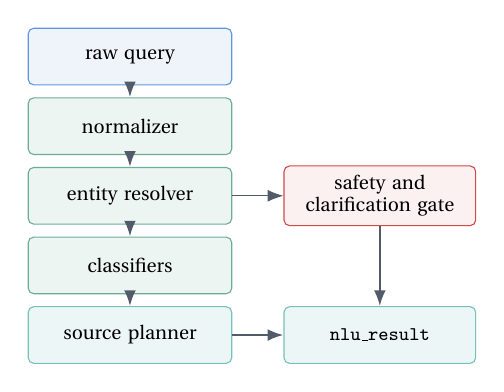
\begin{tikzpicture}[node distance=0.20cm]
        \node[mainbox, text width=2.35cm] (q) {raw query};
        \node[greenbox, below=0.15cm of q, text width=2.35cm] (n) {normalizer};
        \node[greenbox, below=0.15cm of n, text width=2.35cm] (e) {entity resolver};
        \node[greenbox, below=0.15cm of e, text width=2.35cm] (c) {classifiers};
        \node[redbox, right=0.65cm of e, text width=2.2cm] (g) {safety and\\clarification gate};
        \node[tealbox, below=0.15cm of c, text width=2.35cm] (p) {source planner};
        \node[tealbox, right=0.65cm of p, text width=2.2cm] (out) {\texttt{nlu\_result}};
        \draw[flow] (q) -- (n);
        \draw[flow] (n) -- (e);
        \draw[flow] (e) -- (c);
        \draw[softflow] (e) -- (g);
        \draw[flow] (c) -- (p);
        \draw[flow] (g) -- (out);
        \draw[flow] (p) -- (out);
      \end{tikzpicture}
  \end{columns}
\end{frame}

\begin{frame}{Retrieval gathers ranked evidence from documents and APIs}
  \begin{columns}[T,onlytextwidth]
    \column{0.45\textwidth}
      \begin{itemize}
        \item Query builder expands the NLU source plan.
        \item Document retriever returns news, announcements, reports, FAQ, and product docs.
        \item Structured providers return market, fundamental, industry, and macro rows.
        \item Ranker and packager output coverage, warnings, and trace IDs.
      \end{itemize}
    \column{0.51\textwidth}
      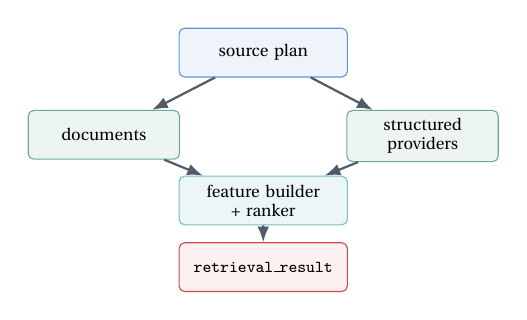
\begin{tikzpicture}[node distance=0.25cm, scale=0.86, transform shape]
        \node[mainbox, text width=2.25cm] (plan) {source plan};
        \node[greenbox, below left=0.48cm and -0.02cm of plan, text width=2.0cm] (doc) {documents};
        \node[greenbox, below right=0.48cm and -0.02cm of plan, text width=2.0cm] (api) {structured\\providers};
        \node[tealbox, below=1.45cm of plan, text width=2.25cm] (rank) {feature builder\\+ ranker};
        \node[redbox, below=0.25cm of rank, text width=2.25cm] (out) {\texttt{retrieval\_result}};
        \draw[flow] (plan) -- (doc);
        \draw[flow] (plan) -- (api);
        \draw[flow] (doc) -- (rank);
        \draw[flow] (api) -- (rank);
        \draw[flow] (rank) -- (out);
      \end{tikzpicture}
  \end{columns}
\end{frame}

\begin{frame}{Market analysis summarizes signals without giving advice}
  \begin{columns}[T,onlytextwidth]
    \column{0.46\textwidth}
      \begin{itemize}
        \item Market signal: returns, MA5/MA20, RSI, MACD, volatility.
        \item Fundamental signal: PE, PB, ROE, and valuation assessment.
        \item Macro signal: available indicators and direction.
        \item Data readiness shows which evidence categories are complete.
      \end{itemize}
    \column{0.50\textwidth}
      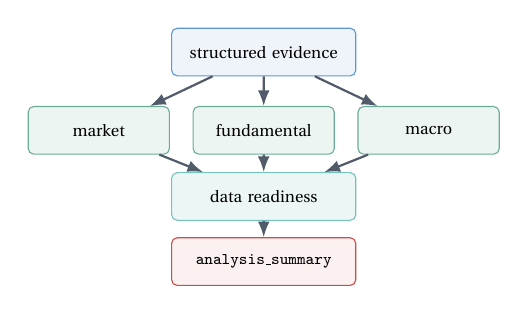
\begin{tikzpicture}[node distance=0.22cm, scale=0.84, transform shape]
        \node[mainbox, text width=2.55cm] (e) {structured evidence};
        \node[greenbox, below left=0.45cm and 0.02cm of e, text width=1.9cm] (m) {market};
        \node[greenbox, below=0.45cm of e, text width=1.9cm] (f) {fundamental};
        \node[greenbox, below right=0.45cm and 0.02cm of e, text width=1.9cm] (ma) {macro};
        \node[tealbox, below=1.45cm of e, text width=2.55cm] (r) {data readiness};
        \node[redbox, below=0.25cm of r, text width=2.55cm] (out) {\texttt{analysis\_summary}};
        \draw[flow] (e) -- (m);
        \draw[flow] (e) -- (f);
        \draw[flow] (e) -- (ma);
        \draw[flow] (m) -- (r);
        \draw[flow] (f) -- (r);
        \draw[flow] (ma) -- (r);
        \draw[flow] (r) -- (out);
      \end{tikzpicture}
  \end{columns}
\end{frame}

\begin{frame}{Sentiment analysis reuses retrieved evidence and entity context}
  \begin{columns}[T,onlytextwidth]
    \column{0.47\textwidth}
      \begin{itemize}
        \item Runs after NLU and retrieval, not as a second understanding system.
        \item Skips out-of-scope, product-info, fee, and missing-entity cases.
        \item Filters documents by source type, language, and entity relevance.
        \item Emits document-level \texttt{SentimentItem} records.
      \end{itemize}
    \column{0.49\textwidth}
      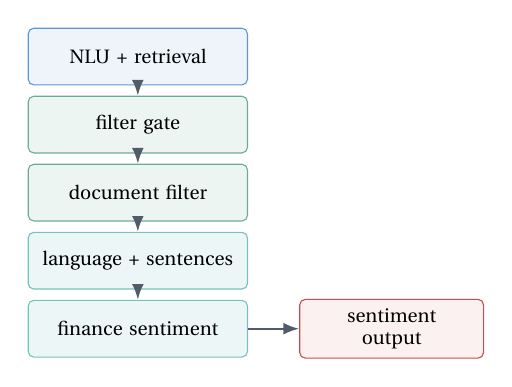
\begin{tikzpicture}[node distance=0.18cm]
        \node[mainbox, text width=2.55cm] (in) {NLU + retrieval};
        \node[greenbox, below=0.13cm of in, text width=2.55cm] (gate) {filter gate};
        \node[greenbox, below=0.13cm of gate, text width=2.55cm] (doc) {document filter};
        \node[tealbox, below=0.13cm of doc, text width=2.55cm] (sent) {language + sentences};
        \node[tealbox, below=0.13cm of sent, text width=2.55cm] (cls) {finance sentiment};
        \node[redbox, right=0.65cm of cls, text width=2.1cm] (out) {sentiment\\output};
        \draw[flow] (in) -- (gate);
        \draw[flow] (gate) -- (doc);
        \draw[flow] (doc) -- (sent);
        \draw[flow] (sent) -- (cls);
        \draw[flow] (cls) -- (out);
      \end{tikzpicture}
  \end{columns}
\end{frame}

\begin{frame}{Answer handoff gives the chatbot validated JSON}
  \begin{columns}[T,onlytextwidth]
    \column{0.47\textwidth}
      \begin{itemize}
        \item Compacts evidence before sending it to the response backend.
        \item Strips raw debug traces and long documents.
        \item Validates \texttt{answer\_generation} and \texttt{next\_question\_prediction}.
        \item Keeps evidence IDs, limitations, and a risk disclaimer.
      \end{itemize}
    \column{0.49\textwidth}
      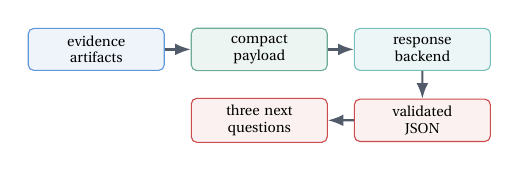
\begin{tikzpicture}[node distance=0.35cm, scale=0.74, transform shape]
        \node[mainbox, text width=2.1cm] (art) {evidence\\artifacts};
        \node[greenbox, right=0.45cm of art, text width=2.1cm] (compact) {compact\\payload};
        \node[tealbox, right=0.45cm of compact, text width=2.1cm] (llm) {response\\backend};
        \node[redbox, below=0.48cm of llm, text width=2.1cm] (json) {validated\\JSON};
        \node[redbox, left=0.45cm of json, text width=2.1cm] (next) {three next\\questions};
        \draw[flow] (art) -- (compact);
        \draw[flow] (compact) -- (llm);
        \draw[flow] (llm) -- (json);
        \draw[flow] (json) -- (next);
      \end{tikzpicture}
  \end{columns}
\end{frame}

\begin{frame}{Current results support the demo story}
  \centering
  \metric{0.9881}{Finance recall}{10k eval}
  \metric{0.9750}{OOD rejection}{10k eval}
  \metric{0.8727}{Intent F1}{10k eval}
  \metric{0.9474}{Topic F1}{10k eval}
  \metric{0.8849}{NDCG@10}{retrieval}

  \vspace{0.7em}
  \begin{tabularx}{0.90\textwidth}{lX}
    \toprule
    Check & Result \\
    \midrule
    Large evaluation & 10,000 bilingual finance and out-of-domain queries; all thresholds passed. \\
    Fuzz matrix & 32/32 cases passed; 361/361 checks passed. \\
    Focused test run & 193 passed, 41 skipped. \\
    \bottomrule
  \end{tabularx}
\end{frame}

\section{Demo and Conclusion}

\begin{frame}{Demo: an English finance query returns grounded evidence}
  \centering
  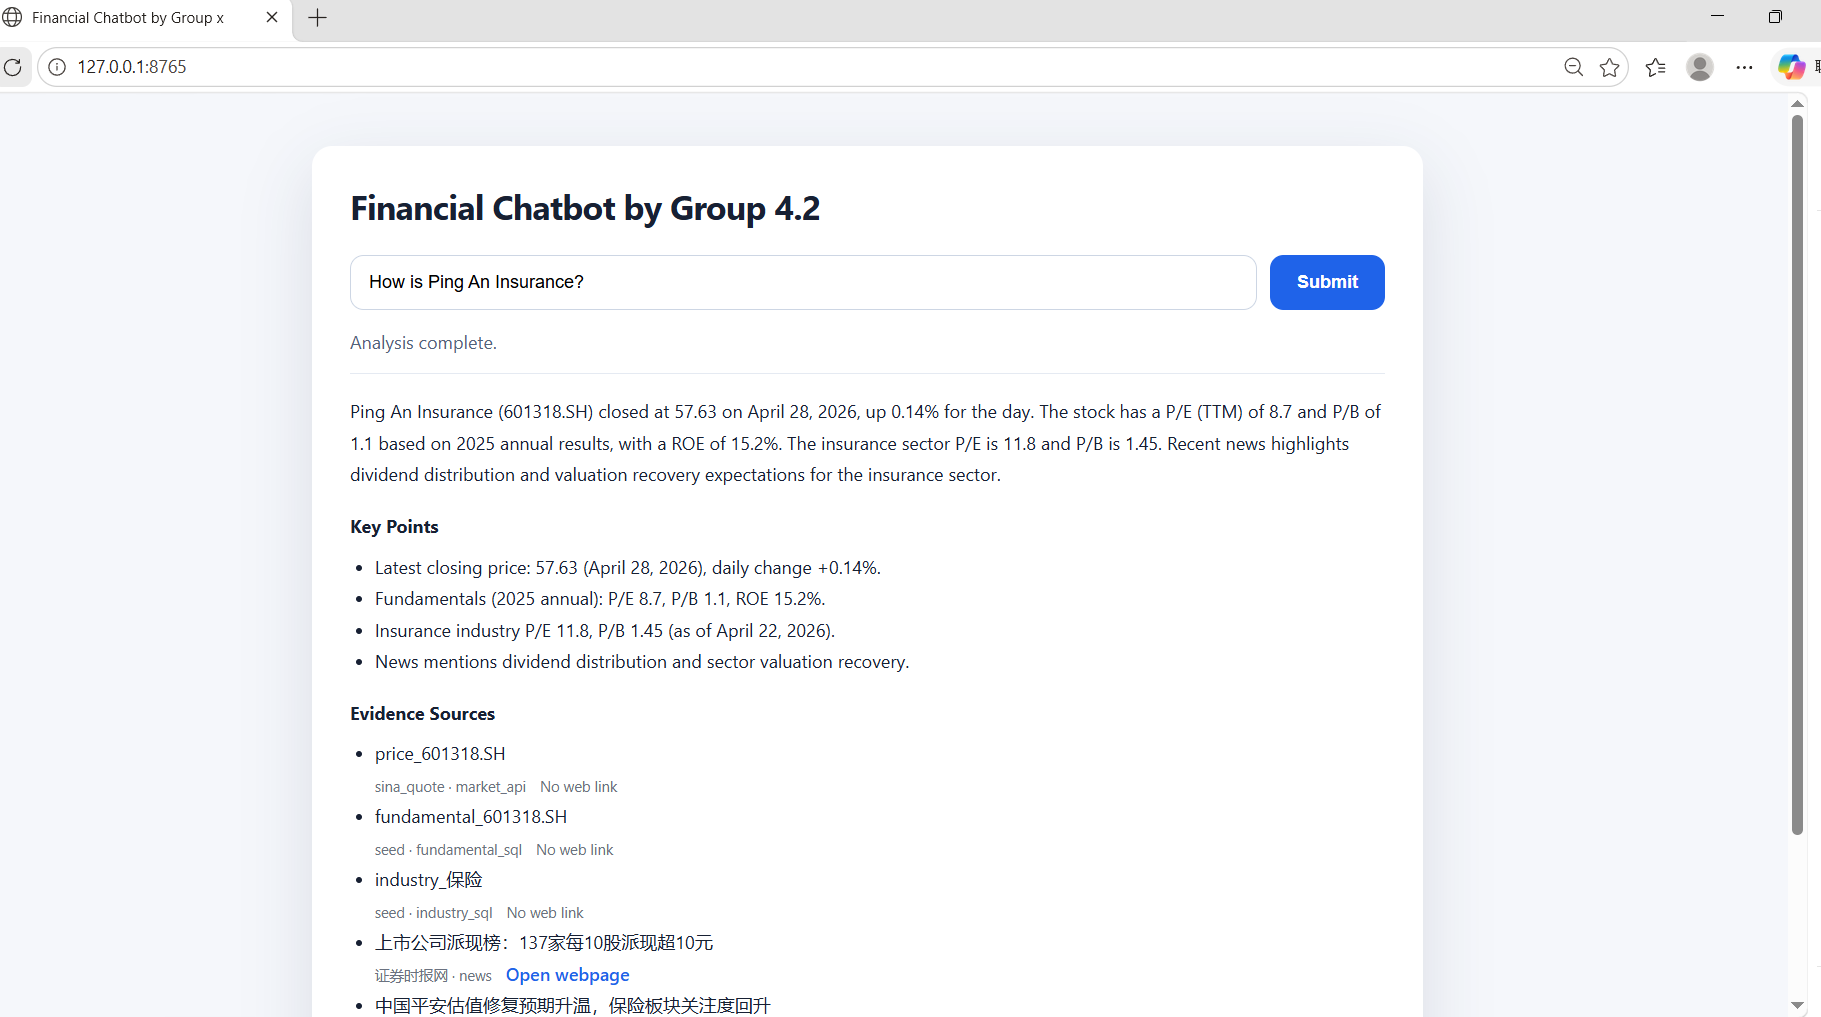
\includegraphics[width=\textwidth,height=0.76\textheight,keepaspectratio]{figures/demo_ping_an.png}

  \slidenote{The answer cites market price, fundamentals, industry valuation, and evidence sources instead of free-form guessing.}
\end{frame}

\begin{frame}{Demo: a Chinese market query uses live price evidence}
  \centering
  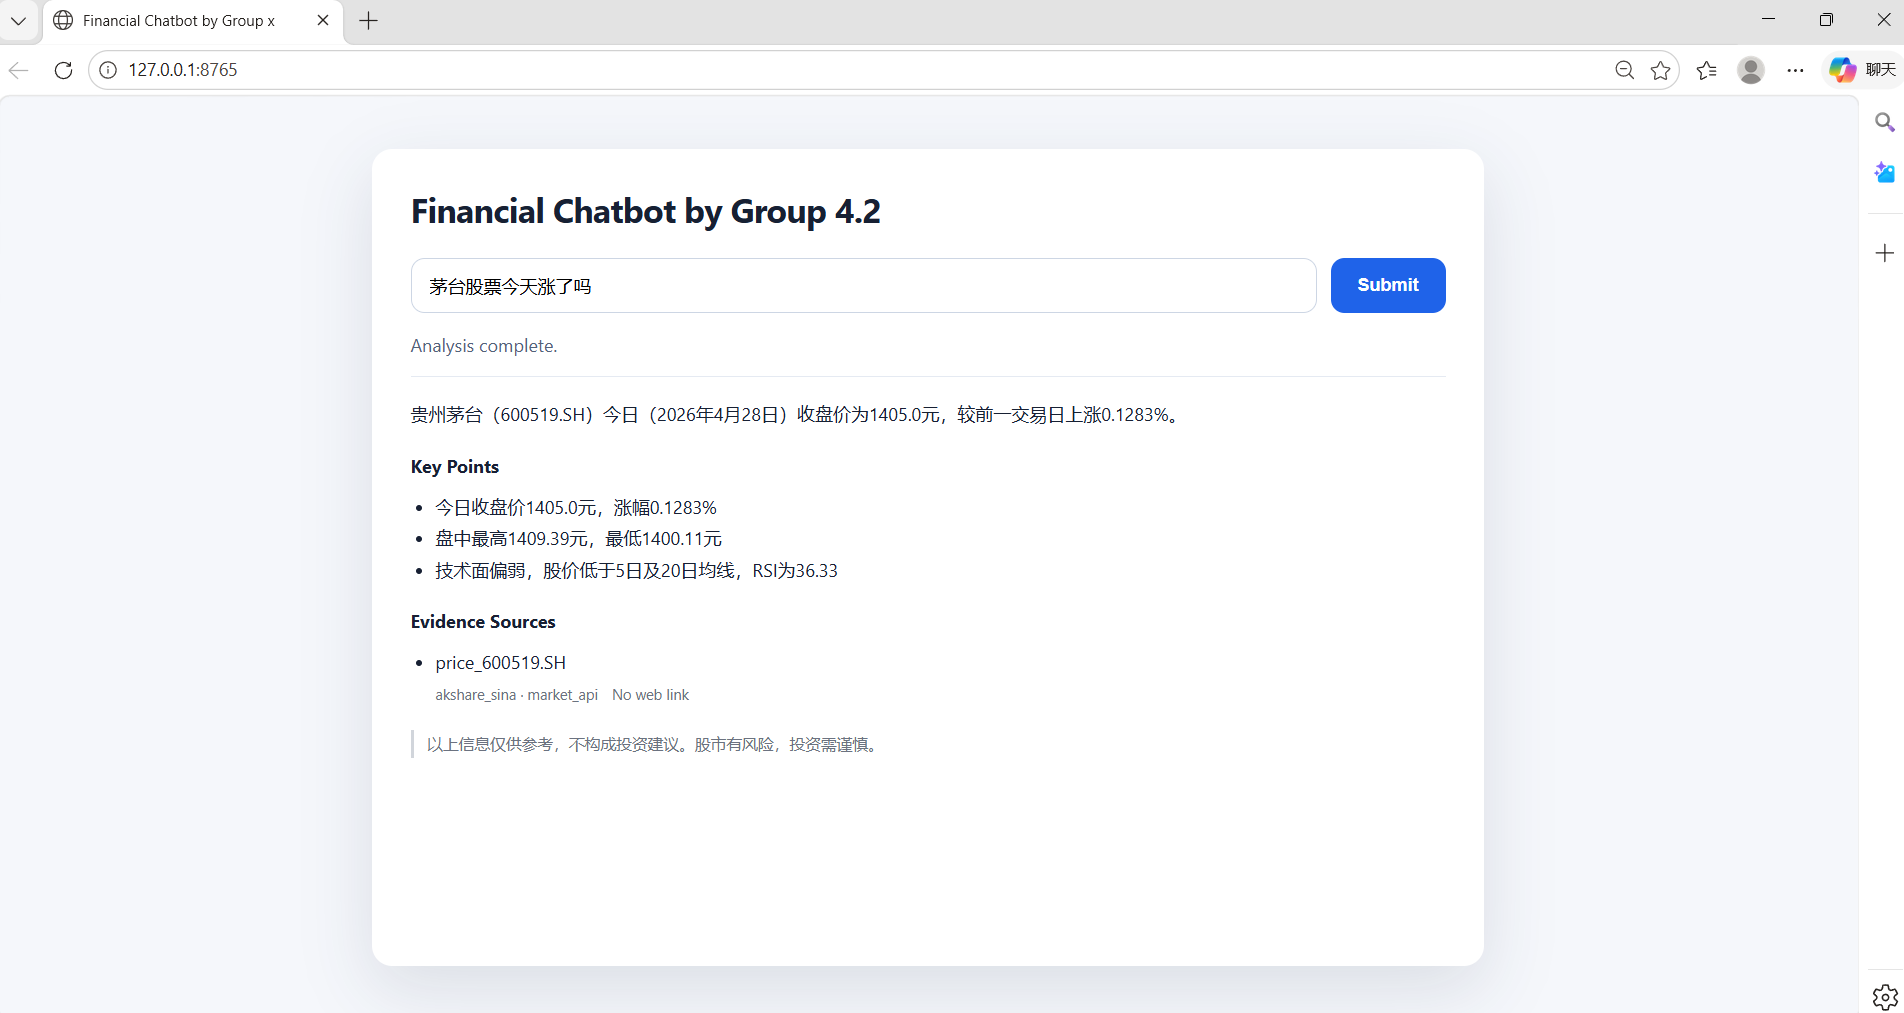
\includegraphics[width=\textwidth,height=0.76\textheight,keepaspectratio]{figures/demo_maotai.png}

  \slidenote{The same pipeline supports Chinese input and returns price movement, intraday range, technical signal, evidence source, and risk disclaimer.}
\end{frame}

\begin{frame}{Demo: an out-of-scope query is rejected safely}
  \centering
  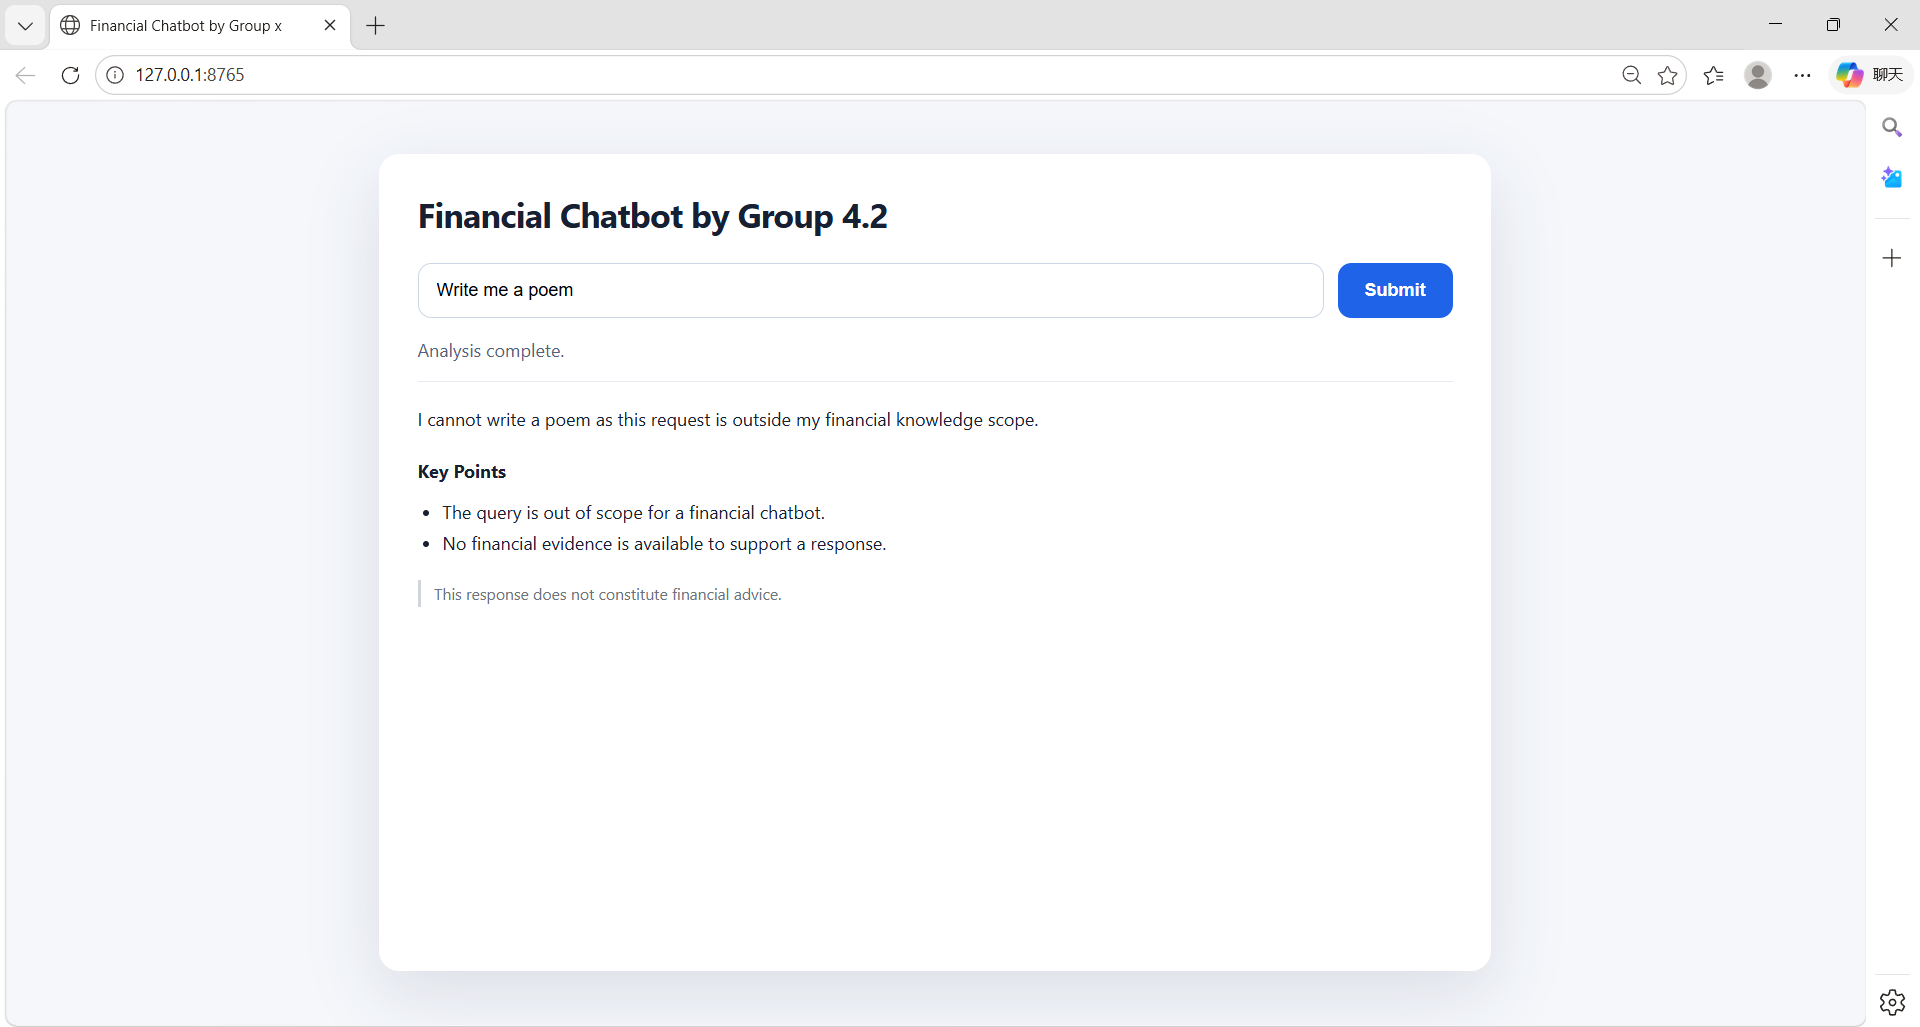
\includegraphics[width=\textwidth,height=0.76\textheight,keepaspectratio]{figures/demo_out_of_scope.png}

  \slidenote{The system detects that the request is not financial and avoids inventing unsupported evidence.}
\end{frame}

\begin{frame}{Future work focuses on integration and robustness}
  \begin{columns}[T,onlytextwidth]
    \column{0.49\textwidth}
      \begin{itemize}
        \item Merge the chatbot frontend with the backend evidence contract.
        \item Extend runtime coverage beyond China-market v1.
        \item Improve live-provider degradation and monitoring.
        \item Add lightweight document sentiment for low-resource deployment.
      \end{itemize}
    \column{0.47\textwidth}
      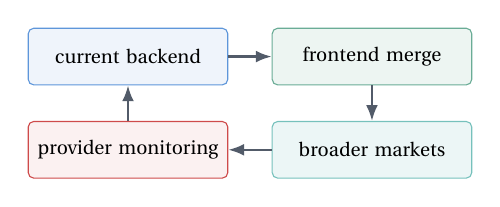
\begin{tikzpicture}[node distance=0.26cm]
        \node[mainbox, text width=2.3cm] (now) {current backend};
        \node[greenbox, right=0.55cm of now, text width=2.3cm] (ui) {frontend merge};
        \node[tealbox, below=0.45cm of ui, text width=2.3cm] (mk) {broader markets};
        \node[redbox, left=0.55cm of mk, text width=2.3cm] (ops) {provider monitoring};
        \draw[flow] (now) -- (ui);
        \draw[flow] (ui) -- (mk);
        \draw[flow] (mk) -- (ops);
        \draw[flow] (ops) -- (now);
      \end{tikzpicture}
  \end{columns}
\end{frame}

\begin{frame}{FinSight makes the chatbot safer and easier to evaluate}
  \begin{itemize}
    \item It separates query understanding, retrieval, analysis, and answer generation.
    \item It keeps the core path classical, inspectable, and measurable.
    \item It gives the chatbot traceable JSON instead of ungrounded guesses.
    \item It supports future UI integration without changing the backend evidence contract.
  \end{itemize}
  \vspace{1em}
  \textcolor{myNewColorA}{\Huge{\centerline{Thank you!}}}
\end{frame}

\end{document}
